\label{FullRecovery3DSection}


This section explains how the Fourier Volume Reconstruction algorithm may be extended to recover full 3D camera pose rotation in addition to translation and scale differences between a pair of captured 3D frames. Proposed is a novel method which uses Principal Components Analysis as a pre-processing step in order to achieve full 3D rotation estimation. For convenience the method is named FVR-3D. Both the FVR method, the FFVR method and the FVR-3D method have unique advantages and disadvantages. FVR is designed to be a robust and efficient method of estimating camera pose and location. It is robust to 3D rotations but cannot register them, if 3D rotation recovery is required, the FVR-3D method discussed in this section provides an efficient solution, but is less robust to noise. The FFVR method may be used with both 3D rotation via PCA pre-processing and without. It is much less robust to noise however it is up to 4 times more efficient for realistic volume sizes. \\

In order to integrate 3D rotation into the standard FVR method, a single axis relating the two 3D models must be known. If such an axis is known prior to executing the FVR method, both 3D frames may be aligned vertically (along the y-axis) with respect to the found axis. Once aligned, the FVR method may be used to register both relative to the final y-axis rotational separation which can be used to recover rotation and scale factors so translation may also be recovered. \\

Several techniques were explored to compute this axis. These include computing the average normal value, the axis defined as the furthest two points and some basic feature matching techniques. The use of Principal Components Analysis (PCA) was also tested. Based on preliminary results PCA was chosen to compute the common axis for use in the FVR-3D method. PCA of course may be used to compute the full rotation separating two 3D frames but this typically fails when noise or non-overlapping parts of the frames are present. To be more robust to noise and non-overlapping features within the frame, only the primary axis is used to align both frames with their primary axis pointing directly up. This is more robust because the primary axis has a stronger presence within the data. This leaves the y-axis rotation to be solved. After which, the full 3D rotation factors may be computed via the FVR method. \\ 

\subsubsection{Computing a Principal Axis}


START HERE:

%Mat m1 = v1.pca_correct_up();
%Mat m2 = v2.pca_correct_up();
%Mat m2i = m2.inv();

%Mat pcm; float rotation, scale; R3 translation;
%phase_correlate_rst(v1, v2, rotation, scale, translation); 
%pcm = VMat::transformation_matrix(v1.s, 0.0f, rotation, 0.0f, scale, translation.x, translation.y, translation.z);
%//un-transform v1 according to the return value of v2's up correction
%//return proper matrix
%return (m2i * pcm * m1);
		

, we can use the most accurate axis (the eigen-vector with the largest corresponding eigen-value) to align two volumes, then y-axis rotation, scale and translation values can be recovered by the described FFT based volume registration method. \\

WARNING: SHOW picture of this PCA procedure

END HERE

Computing the principal axis used in FVR-3D is discussed in this section. As mentioned, PCA is used to compute this axis. Both 3D frames have their axis computed separately before they are used to align both frames to a common axis. To compute the common axis using PCA, both the eigen-values and eigen-vectors of the covariance matrix of the 3D frames must be computed. The eigen-vector with the largest corresponding eigen-value is set to be the primary axis. The procedure works as follows. \\

Given a 3D point cloud $A$ of $N$ points, which may be generated via monocular methods, stereo disparity estimation or active sensor (Kinect, Asus XTion Pro-LIVE), the co-variance of the points between two of the dimensions ($x$ and $y$) is computed as the summation of each $x$ component subtracted by the mean $x$ value multiplied by the $y$ component subtracted by the mean $y$ component value (see equation \ref{eqn:Covariance3DSignal}, $A_{x_{mean}}$ and $A_{y_{mean}}$ refer to the mean values of these x and y dimensions of $A$). \\

\begin{equation} \label{eqn:Covariance3DSignal}
Cov(A_x,A_y) = \sum_{i=0}^{N}(A_{x_i} - A_{x_{mean}})(A_{y_i} - A_{y_{mean}})
\end{equation}

Using the formula for covariance the covariance matrix may be computed for an $N$ dimensional signal. In the case of 3D construction, this matrix is a $3 \times 3$ covariance matrix where each column/row index represents a covariance relationship. This covariance matrix is shown in equation \ref{eqn:CovarMatrix}. This matrix forms a description about how each coordinate axis changes with respect to each other coordinate. The eigen-vectors of this matrix constitute the principal components of the 3D point cloud frame. \\

\begin{equation} \label{eqn:CovarMatrix}
\left[
\begin{array}{ccc}
Cov(A_x, B_x) & Cov(A_x, A_y) & Cov(A_x, A_z) \\
Cov(A_y, B_x) & Cov(A_y, A_y) & Cov(A_y, A_z) \\
Cov(A_z, B_x) & Cov(A_z, A_y) & Cov(A_z, A_z) \\
\end{array}
\right]
\end{equation}

The 3 eigen-vectors of the covariance matrix describe the primary axis of the 3D frame $A$ and the 3 corresponding eigen-values describe the dominance of these vectors. The eigen-vector/axis with the largest corresponding eigen-value is the principal component in PCA and is used as the aligning axis in the FVR-3D method. Here this principal axis is used to align data to a common axis defined to be the vertical y-axis. For simplicity, the principal axis of a 3D frame $A$ is written as $A_{pa}$. During the process of PCA the centroid of the point cloud is also computed. This is simply the average point location within the input point cloud. For simplicity in later discussions, the centroid of a 3D frame $A$ is written as $A_{mean_location}$. A visualization of the principal axis and centroid may be seen in figure WARNING_INSERT_FIGURE_HERE \\

\subsubsection{Alignment Pre-Process}

Using the PCA method, for each input 3D frame $V$, the procedure to compute $V_{pa}$, the principal axis of $V$ computed and used along with the centroid $V_{mean_location}$ to align the input 3D frame using the principal axis $V_{pa}$ as the new vertical axis. To this end, a transformation matrix is formed and is used to rotate the volume such that the principal axis $V_{pa}$ points up. This is useful because if a 3D frame pair are both rotated with respect to their principal axis, and both frames share enough overlap, then only 3D y-axis rotation, 3D translation (and possibly 3D scale) separate the two frames. As discussed in section \ref{Sec:AFVRApproach}, these parameters may be recovered using the FVR method. The matrix used to normalize the 3D frames in terms of their principal axis is discussed here. \\

If $V_{pa}$ (the vector pointing along the principal axis of $V$) is to be set at the new y-axis for the volume, then the other axes must also be computed (x-axis and z-axis). The z-axis, named the forward ($Fwd$) axis is computed based on the cross product between the then x-axis and the principal axis $V_{pa}$ (taken as the y-axis) which gives a psuedo z-axis. The cross product between the principal axis and this pseudo z-axis gives an accurate x-axis. Lastly the cross product between this x-axis and the y-axis (the principal axis) gives the corresponding z-axis in the form of the variable $Fwd$. This is shown in equation \ref{eqn:fwdVector}. \\


\begin{equation} \label{eqn:fwdVector}
Fwd = \left(\left[
\begin{array}{c}
V_{pa_{x}}\\
V_{pa_{y}}\\
V_{pa_{z}}\\
\end{array}
\right] \times \left(\left[
\begin{array}{c}
1\\
0\\
0\\
\end{array}
\right] \times \left[
\begin{array}{c}
V_{pa_{x}}\\
V_{pa_{y}}\\
V_{pa_{z}}\\
\end{array}
\right]\right)\right) \times \left[
\begin{array}{c}
V_{pa_{x}}\\
V_{pa_{y}}\\
V_{pa_{z}}\\
\end{array}
\right]
\end{equation}

The final axis completing the new space is the x-axis defined at the cross product between the principal axis (the new y-axis) and the z-axis (the $Fwd$ vector) and is named $Rgt$ (standing for right facing axis). Equation \ref{eqn:rgtVector} shows this calculation. This completes the new space defined by x-axis $Rgt$, y-axis $V_{pa}$ and z-axis $Fwd$. A rotation matrix transforming original space to the new space given by these axes may be computed using the $Rgt$, $V_{pa}$ and $Fwd$ axes as the column vectors of the rotation matrix. The inverse, that is the transformation from the new space to the original space may computed using the transpose of that rotation matrix. The rotation of the point cloud from the new space defined by the principal axis to the original space is useful as it aligns the principal axis to the y-axis leaving only 3D y-axis rotation, 3D translation and possibly scale to be registered. \\ 


\begin{equation} \label{eqn:rgtVector}
Rgt = \left[
\begin{array}{c}
V_{pa_{x}}\\
V_{pa_{y}}\\
V_{pa_{z}}\\
\end{array}
\right] \times \left[
\begin{array}{c}
Fwd_x\\
Fwd_y\\
Fwd_z\\
\end{array}
\right]
\end{equation}

The input 3D frame $V$ may be aligned by its principal axis as the new y-axis by first transforming the centroid to the origin. Next the 3D frame may be rotated from the new space to the default identity space. This sets $Rgt$ to be the new x-axis, $V_{pa}$ to be the new y-axis and $Fwd$ to be the new z-axis. The rotation matrix may be computed as the row vectors of these axes. Finally, after the rotation the 3D frame $V$ may be transformed back to the centroid. This aligns the 3D frame so that $V_{pa}$ points towards the y-axis. The compounded transformation to perform this alignment is fully defined in equation \ref{eqn:CorrectUpMat}. \\

\begin{equation} \label{eqn:CorrectUpMat}
CorrectMat(V) = \left[
\begin{array}{cccc}
1 & 0 & 0 & V_{mean_x} \\
0 & 1 & 0 & V_{mean_y} \\
0 & 0 & 1 & V_{mean_z} \\
0 & 0 & 0 & 1 \\
\end{array}
\right] \left[
\begin{array}{cccc}
Rgt_x & Rgt_y & Rgt_z & 0 \\
V_{pa_x} & V_{pa_y} & V_{pa_z} & 0 \\
Fwd_x & Fwd_y & Fwd_z & 0 \\
0 & 0 & 0 & 1 \\
\end{array}
\right] \left[
\begin{array}{cccc}
1 & 0 & 0 & -V_{mean_x} \\
0 & 1 & 0 & -V_{mean_y} \\
0 & 0 & 1 & -V_{mean_z} \\
0 & 0 & 0 & 1 \\
\end{array}
\right]
\end{equation}

\subsubsection{3D Rotation Registration}

To recover a matrix for full 3D rotation separating two input 3D frames $A$ and $B$ which have been taken from two different locations (translation separation) with two different poses (3D rotational separation) and possibly projected differently (scale separation), the first step is to align both frames by their principal axis. The alignment matrix for $A$ can be computed as $C_A = CorrectMat(A)$ and the alignment matrix for $B$ may be computed as $C_B = CorrectMat(B)$. Transforming both $A$ and $B$ by their alignment matrix gives two volumes $A_{aligned} = Transform(A, C_A)$ and $B_{aligned} = Transform(B, C_B)$ which are now only separated by 3D y-axis rotation, 3D translation and 3D scaling factors. As discussed in sections \ref{Sec:VolumeRegistrationSection} and \ref{Sec:AFVRApproach} these factors may be computed and a registration matrix aligning $A_{aligned}$ and $B_{aligned}$. This matrix is computed as $R_{y}ST = FVR(A_{aligned},B_{aligned})$. Using this registration matrix and the alignment matrices $C_{A}$ and $C_{B}$, the full 3D rotation, 3D scale and 3D translation registration matrix, $R_{x,y,z}ST$ transforming $A$ to $B$ may be computed may be recovered as the the matrix which aligns $A$, registers it using $R_{y}ST$ (which aligns it with $B_{aligned}$) then inverse transforms it by $C_{B}$ which un-aligns it according to the alignment matrix $C_B$. This can be followed as in equation \ref{eqn:FullRSTTransform}. \\ 

\begin{equation} \label{eqn:FullRSTTransform}
R_{x,y,z}ST Matrix = C_{B}^{-1} \times R_{y}ST \times C_A
\end{equation}

This explanation completes the FVR-3D technique. FVR-3D is a capable registration method which extends Fourier registration to take into account full 3D rotation. The complexity of the technique adds a single layer of complexity over the FVR method. For the additional computational complexity is primarily made up of computing the covariance matrix, which adds a complexity of $N^3$ which is minimal compared to the rest of the FVR technique. \\

WARNING: show an example of this working

\subsubsection{Pipeline}

\label{METHOD_SECLL}
The proposed 3D reconstruction method consists of various steps. First each frame $f_i$ that is captured, consisting of a colour and depth image pair is projected into 3D space, forming colour point cloud $points_i$ and re-sampled into a volume $V_i$. Then, the transform parameters between pairs of volumes $V_i$ and $V_{i+1}$ are estimated using $VolumeRegister_{\theta \varphi t_x t_y t_z}$ shortened to $VR_{\theta \varphi t_x t_y t_z}$. These parameters are used to update transformation matrix $M$. The points corresponding to $f_2$ ($points_1$) are then transformed using the updated $M$ matrix and added to the cumulative $PointCloud$ database. Two lists, $Cameras$ and $Poses$, are also updated to track camera pose and location per frame. This basic procedure is given in listings \ref{algorithm:PCSLAM} and elaborated upon in subsequent subsections.
\begin{figure}
\begin{lstlisting}[language=c++,caption=Phase Correlation Based SLAM Algorithm,label=algorithm:PCSLAM,mathescape,basicstyle=\ttfamily]
$f_1$ = ReadFrame();
$PointCloud$ = project($f_1$);
$M$ = IdentityMatrix();
$Camera$ = $[0, 0, 0]^T$;
$Pose$ = $[0, 0, 1]^T$;
$Cameras$ = $\left[Camera\right]$, $Poses$ = $\left[Pose\right]$;
while(more frames){
	$f_2$ = ReadFrame();
	$points_1$ = project($f_2$);
	$points_2$ = project($f_1$);
	$V_1$ = ResampleVolume($points_1$);
	$V_2$ = ResampleVolume($points_2$);
	$(\theta, \varphi, t_x, t_y, t_z) = VR_{\theta \varphi t_x t_y t_z}(V_1, V_2)$;
	$M = M \times$TransformMat($(\theta, \varphi, t_x, t_y, t_z)$);
	$points_1$ = Transform($points_1$, $M$);
	$PointCloud$ = $PointCloud \cup points_1$;
	$Camera$ = $M^{-1} \times Camera$;
	$Pose$ = $M^{-1} \times Pose$;
	$Cameras.add(Camera)$;
	$Poses.add\left(\frac{Pose-Camera}{|Pose-Camera|}\right)$;
	$f_1$ = $f_2$;
}
\end{lstlisting}
\end{figure}


The input to our method is a color and depth image pair, $f(u,v)$ and $g(u,v)$ obtained using an Asus Xtion PRO LIVE sensor at a resolution of $640 \times 480$. Each pixel is projected into 3D space using $X_{u,v} = \frac{(u - c_x)Z_{u,v}}{f}$, $Y_{u,v} = \frac{(v - c_y)Z_{u,v}}{f}$ and $Z_{u,v}$ = $g(u,v)$. 
Here, $[c_x c_y]^T$ represent the center of the image whilst $f$ represents the focal length, defined as $525.0$. The point clouds generated by projecting these images are then quantized into image volumes. Results reported in this paper were obtained using volumes of $384^3$ voxels in size.

\begin{figure*}[!htb]
\centering
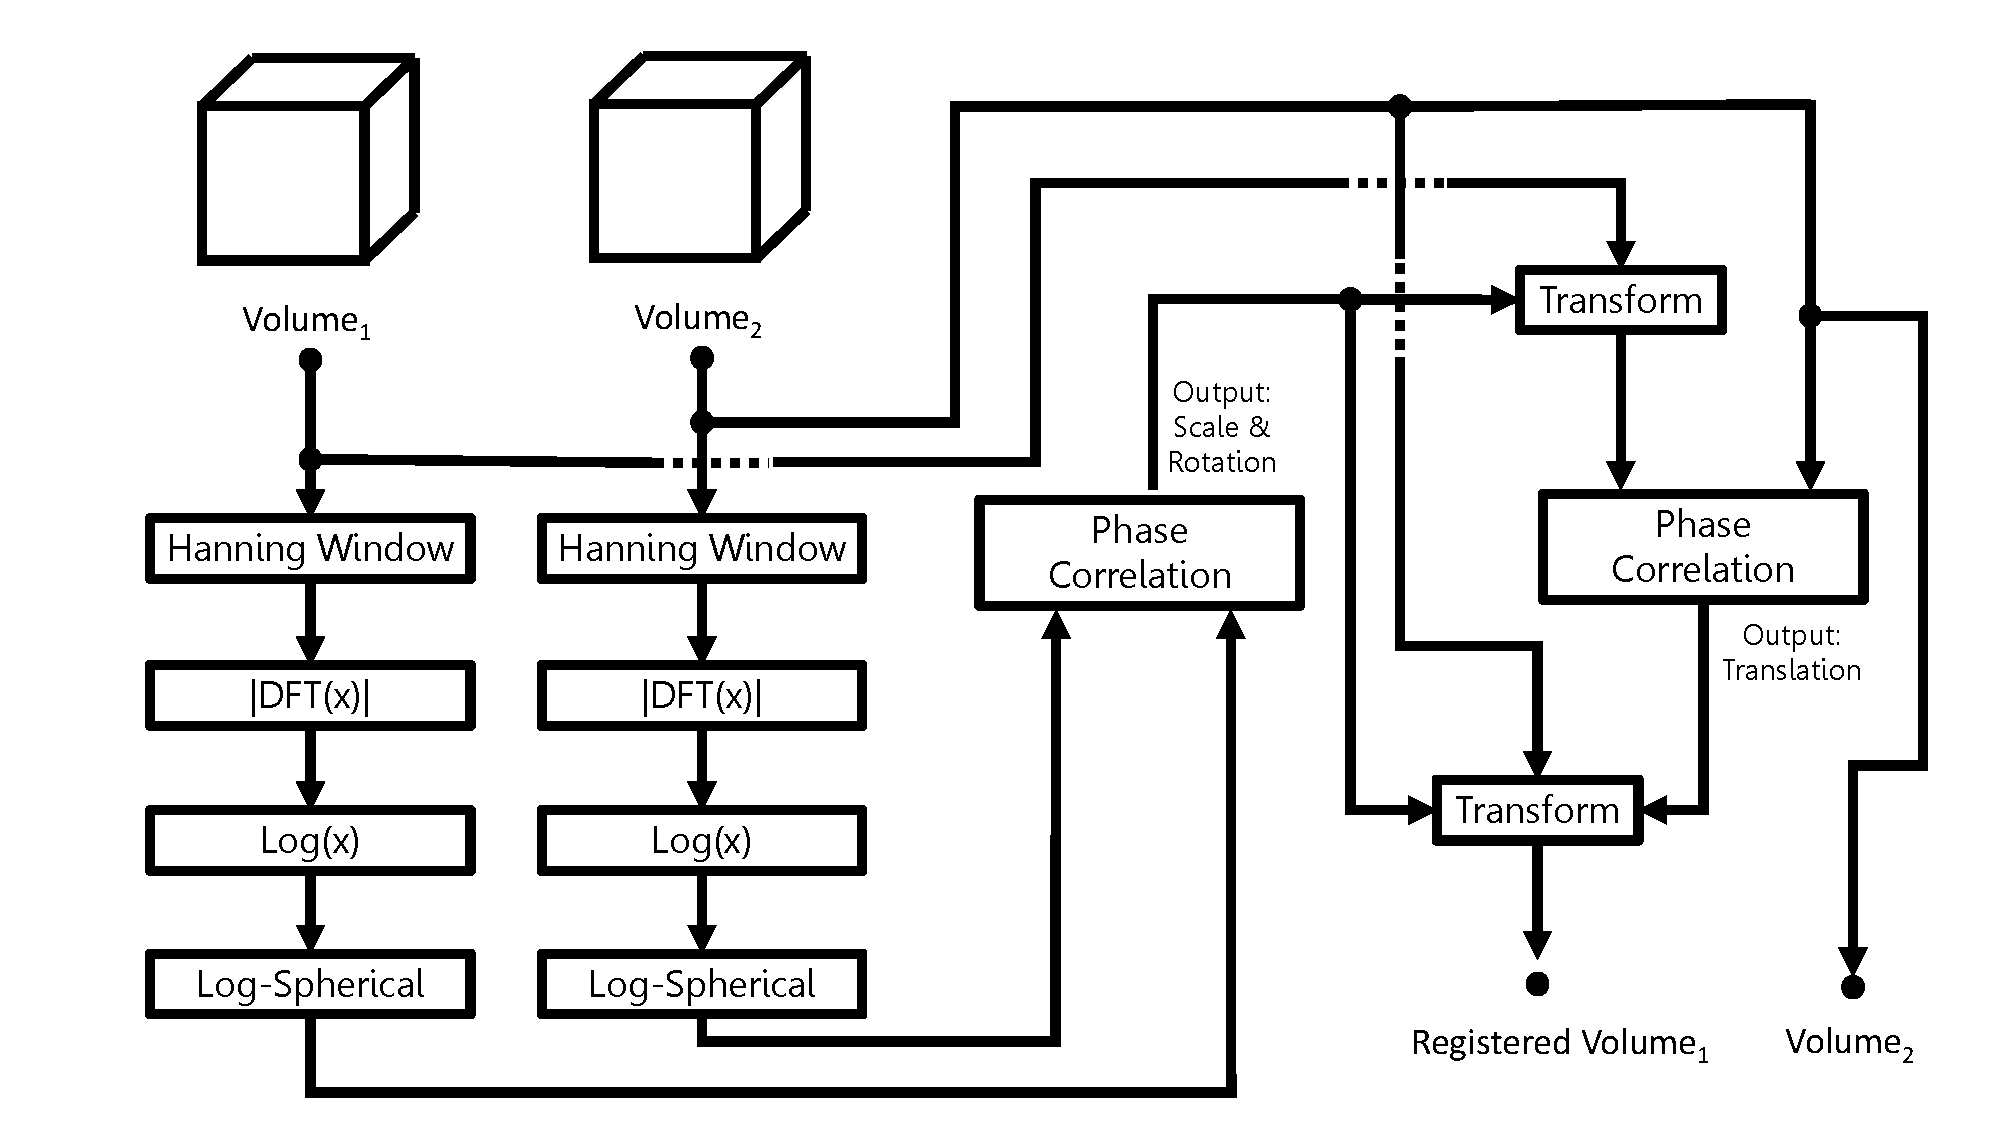
\includegraphics[width=6.0in]{images/ch2/pipeline2}
\caption{System Diagram for Registration Process}
\label{fig:PIPELINE}
\end{figure*}


\subsubsection{Error metrics}

\label{metricsSection}

In order to evaluate the accuracy of volume registration we use several error metrics including: Hausdorff error, mean squared error and the percentage of matched voxels. We describe mathematically those techniques here. All measurements are based on a simple function which computes the nearest neighbour for a given 3D point or voxel given a volume (or collection of 3D points). We define such a function, named nearest-neighbour in equation \ref{eqn:NN}.

\begin{equation} \label{eqn:NN}
NN(p, V) =  \{ q \in V | (Dist(q, p) < Dist(k, p))  \forall k \in V \}
\end{equation}

This function retrieves the closest corresponding point given a query point $p$ and a volume or point cloud of points, $V$. This function can be used to provide omni-directional error functions based on Hausdorff, mean squared and percentage accuracy error metrics.

Here some one-way error functions are described. The one was Hausdorff error is defined in \ref{eqn:HDOW} 

\begin{equation} \label{eqn:HDOW}
\sum_{k=0}^{N} Dist(P_k, NN(P_k, Q))
\end{equation}

\subsubsection{Reconstruction Integration}

Using the techniques of registration described in the above sections, there are several techniques which may be used to integrate these registered data. In most experiments we use the volume integration to combine the registered data in a single global model. We also propose several techniques for data representation and evaluate their abilities (see section \ref{sec:3DDataRepresentations}). As for the typical volume integration used, we create volumes with dimensions of $512\times 512\times 512$, although larger sizes may be used for increased accuracy. Once a frame is registered, it is projected into the volume. \\

This projection follows the following formula


\begin{equation} \label{eqn:volIntegration}
\begin{split}
x^{1} & = floor((x - frameCenter_x) \times scalar + volumeCenter_x) \\
y^{1} & = floor((y - frameCenter_y) \times scalar + volumeCenter_y) \\
z^{1} & = floor((z - frameCenter_z) \times scalar + volumeCenter_z)
\end{split}
\end{equation}

$frameCenter$ is the center of the projected frame space and $volumeCenter$ is the center of the integration volume, typically scalar is set to 1 or is used to trade-off resolution and map size. An example of an integration process is illustrated in figure XFDF. 





